\documentclass[10pt, aspectratio=169]{beamer}

% --- THEME & STYLING ---
\usetheme{Madrid}
\usecolortheme{whale}

% --- PACKAGES ---
\usepackage[utf8]{inputenc}
\usepackage{amsmath, amssymb, amsfonts}
\usepackage{booktabs}
\usepackage{graphicx}
\usepackage{hyperref}
\usepackage{tikz}
\usetikzlibrary{shapes.geometric, arrows, positioning}
\usepackage{xcolor}

% --- CUSTOM COLOR DEFINITIONS ---
\definecolor{DeepNavy}{RGB}{15, 23, 42}
\definecolor{AccentTeal}{RGB}{15, 118, 110}
\definecolor{SkyBlue}{RGB}{56, 189, 248}
\definecolor{CardBg}{RGB}{248, 250, 252}

\setbeamercolor{palette primary}{bg=DeepNavy, fg=white}
\setbeamercolor{palette secondary}{bg=AccentTeal, fg=white}
\setbeamercolor{palette tertiary}{bg=DeepNavy!90, fg=white}
\setbeamercolor{titlelike}{parent=palette primary}
\setbeamercolor{structure}{fg=AccentTeal}
\setbeamercolor{block title}{bg=DeepNavy, fg=white}
\setbeamercolor{block body}{bg=CardBg, fg=DeepNavy}

% --- PRESENTATION METADATA ---
\title[BDA Suicide Analytics]{Global Socio-Demographic \& Suicide Analytics}
\subtitle{Big Data Engineering, Exploratory Analytics, and Predictive ML Pipeline}
\author[Ayush]{
    \textbf{Team Members:} Ayush \\
    \vspace{0.15cm}
    \small \textbf{Project Guide:} Faculty Mentor / Guide
}
\institute[Dept. of CSE]{
    Department of Computer Science \& Engineering \\
    Course: Big Data Analytics (BDA) --- Academic Year 2025--2026
}
\date{\today}

\begin{document}

% ==============================================================================
% SLIDE 1: TITLE, TEAM MEMBERS AND GUIDE
% ==============================================================================
\begin{frame}[plain]
    \titlepage
\end{frame}

% ==============================================================================
% SLIDE 2: PROBLEM STATEMENT AND MOTIVATION
% ==============================================================================
\begin{frame}{Slide 2: Problem Statement \& Motivation}
    \begin{columns}[T]
        \begin{column}{0.48\textwidth}
            \begin{block}{\textbf{Problem Statement}}
                \begin{itemize}
                    \item Suicide is a multifaceted global crisis with profound socio-demographic roots.
                    \item Traditional public health reporting relies on \textbf{static, retrospective census tables} that fail to:
                    \begin{itemize}
                        \item Scale across heterogeneous multi-national cohorts.
                        \item Dynamically identify cross-demographic vulnerability disparities.
                        \item Provide proactive, real-time predictive risk assessment.
                    \end{itemize}
                \end{itemize}
            \end{block}
        \end{column}
        \begin{column}{0.48\textwidth}
            \begin{block}{\textbf{Motivation}}
                \begin{itemize}
                    \item \textbf{Preventable Loss of Life:} Suicide mortality can be mitigated with timely, targeted public health interventions.
                    \item \textbf{Big Data Opportunity:} Leveraging demographic, economic (GDP), and development (HDI) features allows automated prioritization of vulnerable cohorts.
                    \item \textbf{Actionable Delivery:} Bridging complex statistical learning with an accessible, interactive web dashboard.
                \end{itemize}
            \end{block}
        \end{column}
    \end{columns}
\end{frame}

% ==============================================================================
% SLIDE 3: OBJECTIVES
% ==============================================================================
\begin{frame}{Slide 3: Project Objectives}
    \begin{columns}[T]
        \begin{column}{0.5\textwidth}
            \begin{block}{\textbf{Primary Engineering Objectives}}
                \begin{enumerate}
                    \item \textbf{Scalable Data Preprocessing:} Design an automated pipeline for schema normalization, missing value imputation, and Interquartile Range (IQR) outlier diagnostics.
                    \item \textbf{Distributed Computing Simulation:} Implement a Big Data \textbf{MapReduce} architecture demonstrating partitioned Map, Shuffle \& Sort, and Reduce aggregations.
                \end{enumerate}
            \end{block}
        \end{column}
        \begin{column}{0.5\textwidth}
            \begin{block}{\textbf{Machine Learning \& Deployment Objectives}}
                \begin{enumerate}
                    \setcounter{enumi}{2}
                    \item \textbf{Predictive ML Suite:} Train and benchmark:
                    \begin{itemize}
                        \item \textbf{Supervised Regression:} Predict continuous suicide rates per 100k.
                        \item \textbf{Supervised Classification:} Categorize cohorts into 3 risk tiers (\textit{Low, Moderate, High}).
                        \item \textbf{Unsupervised Clustering:} K-Means and 2D PCA for demographic segmentation.
                    \end{itemize}
                    \item \textbf{Interactive Dashboard:} Deploy a full-stack Streamlit web application with real-time \textit{What-If} scenario prediction.
                \end{enumerate}
            \end{block}
        \end{column}
    \end{columns}
\end{frame}

% ==============================================================================
% SLIDE 4: EXISTING SYSTEM / LITERATURE REVIEW
% ==============================================================================
\begin{frame}{Slide 4: Existing System \& Literature Review}
    \begin{columns}[T]
        \begin{column}{0.48\textwidth}
            \begin{block}{\textbf{Existing System Architecture}}
                \begin{itemize}
                    \item Traditional WHO and CDC health surveillance relies on \textbf{annual batch PDF/Excel releases}.
                    \item Relies on isolated relational databases without distributed preprocessing mechanisms.
                    \item Lack of machine learning-driven risk forecasting or scenario simulation.
                \end{itemize}
            \end{block}
            \begin{alertblock}{\textbf{Limitations of Existing Approaches}}
                \begin{itemize}
                    \item High processing latency on large datasets.
                    \item Rigid schema structures; unable to handle streaming data.
                    \item No personalized or cohort-level What-If forecasting.
                \end{itemize}
            \end{alertblock}
        \end{column}
        \begin{column}{0.48\textwidth}
            \begin{block}{\textbf{Literature Review \& Research Gaps}}
                \begin{itemize}
                    \item \textbf{Socio-Demographic Disparities:} Prior studies establish severe gender and age asymmetries in mortality rates.
                    \item \textbf{Big Data Analytics in Healthcare:} Demonstrated efficacy of distributed MapReduce paradigms for epidemiological cubes.
                    \item \textbf{Identified Gap:} Lack of unified end-to-end pipelines connecting automated Big Data preprocessing, ML classification, and real-time interactive user interfaces.
                \end{itemize}
            \end{block}
        \end{column}
    \end{columns}
\end{frame}

% ==============================================================================
% SLIDE 5: PROPOSED SYSTEM AND METHODOLOGY
% ==============================================================================
\begin{frame}{Slide 5: Proposed System \& Methodology}
    \begin{columns}[T]
        \begin{column}{0.5\textwidth}
            \begin{block}{\textbf{Methodological Framework}}
                \begin{enumerate}
                    \item \textbf{Phase 1: Ingestion \& Profiling} \\
                    Ingest multi-country records (\texttt{master.csv}); validate data types, memory footprint, and null counts.
                    \item \textbf{Phase 2: Cleaning \& Transformation} \\
                    Standardize column naming; apply median imputation for socioeconomic indicators ($\hat{x}_{\text{HDI}} = \text{Median}(X)$); compute IQR boundaries for outlier diagnostics.
                    \item \textbf{Phase 3: Feature Engineering} \\
                    Derive normalized rate: $\text{Rate}_{100k} = (\frac{\text{Cases}}{\text{Pop}}) \times 10^5$; map age ordinally; assign 3-tier risk labels.
                \end{enumerate}
            \end{block}
        \end{column}
        \begin{column}{0.5\textwidth}
            \begin{block}{\textbf{Analytical \& Modeling Methodology}}
                \begin{enumerate}
                    \setcounter{enumi}{3}
                    \item \textbf{Phase 4: Distributed Processing} \\
                    Chunk-based MapReduce simulation for group-level rate aggregations.
                    \item \textbf{Phase 5: Predictive ML Training} \\
                    Multi-model regression and classification with train/test validation (75:25) and feature scaling (\texttt{StandardScaler}).
                    \item \textbf{Phase 6: Interactive Deployment} \\
                    Streamlit interface with Plotly graphics and live What-If predictive simulation.
                \end{enumerate}
            \end{block}
        \end{column}
    \end{columns}
\end{frame}

% ==============================================================================
% SLIDE 6: SYSTEM ARCHITECTURE / WORKFLOW / DESIGN
% ==============================================================================
\begin{frame}{Slide 6: System Architecture \& Workflow Design}
    \centering
    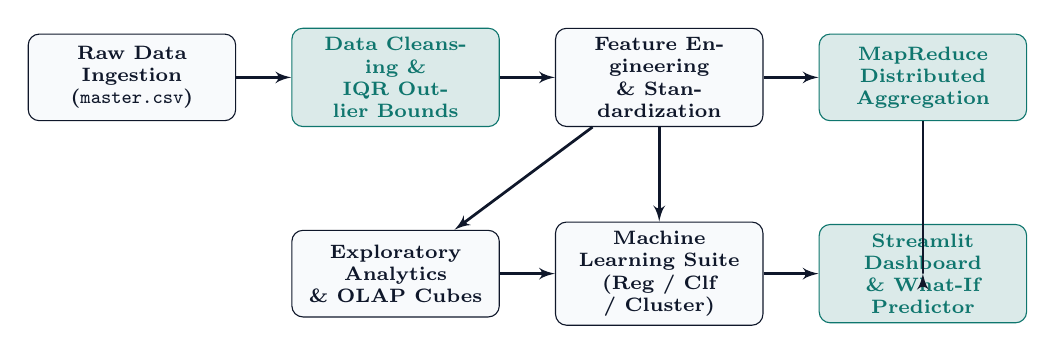
\begin{tikzpicture}[node distance=1.1cm, auto,
        block/.style={rectangle, draw=DeepNavy, fill=CardBg, text=DeepNavy, text width=2.4cm, text centered, rounded corners, minimum height=1.1cm, font=\scriptsize\bfseries},
        accent/.style={rectangle, draw=AccentTeal, fill=AccentTeal!15, text=AccentTeal, text width=2.4cm, text centered, rounded corners, minimum height=1.1cm, font=\scriptsize\bfseries},
        line/.style={draw=DeepNavy, -latex', line width=1pt}]
        
        % Nodes
        \node [block] (raw) {Raw Data Ingestion\\(\texttt{master.csv})};
        \node [accent, right=0.7cm of raw] (clean) {Data Cleansing \&\\IQR Outlier Bounds};
        \node [block, right=0.7cm of clean] (feat) {Feature Engineering\\\& Standardization};
        \node [accent, right=0.7cm of feat] (mr) {MapReduce\\Distributed Aggregation};
        
        \node [block, below=1.2cm of feat] (ml) {Machine Learning Suite\\(Reg / Clf / Cluster)};
        \node [accent, right=0.7cm of ml] (dash) {Streamlit Dashboard\\\& What-If Predictor};
        \node [block, left=0.7cm of ml] (olap) {Exploratory Analytics\\\& OLAP Cubes};
        
        % Paths
        \path [line] (raw) -- (clean);
        \path [line] (clean) -- (feat);
        \path [line] (feat) -- (mr);
        \path [line] (feat) -- (ml);
        \path [line] (feat) -- (olap);
        \path [line] (ml) -- (dash);
        \path [line] (mr) |- (dash);
        \path [line] (olap) -- (ml);
    \end{tikzpicture}
    
    \vspace{0.3cm}
    \begin{columns}[T]
        \begin{column}{0.32\textwidth}
            \textbf{1. Data Ingestion Layer:} Schema validation \& type casting.
        \end{column}
        \begin{column}{0.32\textwidth}
            \textbf{2. Processing \& ML Layer:} MapReduce chunking \& multi-model training.
        \end{column}
        \begin{column}{0.32\textwidth}
            \textbf{3. Presentation Layer:} Streamlit UI with real-time inference.
        \end{column}
    \end{columns}
\end{frame}

% ==============================================================================
% SLIDE 7: IMPLEMENTATION – MODULES AND TECHNOLOGIES
% ==============================================================================
\begin{frame}{Slide 7: Implementation --- Modules \& Technologies}
    \begin{columns}[T]
        \begin{column}{0.48\textwidth}
            \begin{block}{\textbf{Core Software Modules}}
                \begin{itemize}
                    \item \texttt{src/data\_loader.py}: Ingestion and distributed MapReduce chunking engine.
                    \item \texttt{src/preprocessing.py}: Data cleaning, median imputation, IQR outliers, feature engineering, and scaling.
                    \item \texttt{src/ml\_models.py}: ML suite (Regression, Classification, K-Means, and Real-Time Predictor).
                    \item \texttt{src/bda\_analytics.py}: Multi-dimensional OLAP rollups and Demographic Vulnerability Index (DVI).
                    \item \texttt{app.py}: Full Streamlit interactive dashboard.
                \end{itemize}
            \end{block}
        \end{column}
        \begin{column}{0.48\textwidth}
            \begin{block}{\textbf{Technology Stack}}
                \begin{itemize}
                    \item \textbf{Core Language:} Python 3.13
                    \item \textbf{Data Processing:} Pandas 2.3, NumPy 2.2
                    \item \textbf{Machine Learning:} Scikit-learn 1.9 (Regression, Ensembles, Clustering, PCA)
                    \item \textbf{Visualization:} Plotly 7.1 (Dynamic charts, maps, heatmaps, matrices)
                    \item \textbf{Web Framework:} Streamlit 1.64 \& Streamlit Option Menu
                    \item \textbf{Version Control \& Cloud:} Git, GitHub, Streamlit Community Cloud
                \end{itemize}
            \end{block}
        \end{column}
    \end{columns}
\end{frame}

% ==============================================================================
% SLIDE 8: RESULTS, SCREENSHOTS AND PERFORMANCE
% ==============================================================================
\begin{frame}{Slide 8: Results, Benchmarks \& Performance}
    \begin{columns}[T]
        \begin{column}{0.5\textwidth}
            \begin{block}{\textbf{Supervised Regression Benchmarks}}
                \begin{table}[h]
                    \centering
                    \scriptsize
                    \begin{tabular}{@{}lccc@{}}
                        \toprule
                        \textbf{Algorithm} & \textbf{$R^2$ Score} & \textbf{RMSE} & \textbf{MAE} \\ \midrule
                        \textbf{Decision Tree Regressor} & \textbf{0.929} & \textbf{8.10} & \textbf{5.73} \\
                        Linear Regression & 0.813 & 13.14 & 10.53 \\
                        Random Forest Regressor & 0.788 & 14.01 & 11.20 \\ \bottomrule
                    \end{tabular}
                \end{table}
            \end{block}
            \begin{block}{\textbf{Supervised Classification Benchmarks}}
                \begin{table}[h]
                    \centering
                    \scriptsize
                    \begin{tabular}{@{}lccc@{}}
                        \toprule
                        \textbf{Algorithm} & \textbf{Accuracy} & \textbf{Precision} & \textbf{F1} \\ \midrule
                        \textbf{Decision Tree Classifier} & \textbf{87.5\%} & \textbf{0.90} & \textbf{0.87} \\
                        Logistic Regression & 50.0\% & 0.58 & 0.48 \\
                        Random Forest Classifier & 50.0\% & 0.55 & 0.50 \\ \bottomrule
                    \end{tabular}
                \end{table}
            \end{block}
        \end{column}
        \begin{column}{0.48\textwidth}
            \begin{block}{\textbf{Unsupervised Clustering \& PCA ($k=3$)}}
                \begin{itemize}
                    \item \textbf{PC1 \& PC2:} Account for $>65\%$ feature variance.
                    \item \textbf{Cluster 0 (Senior High-Risk):} Peak rates ($>75/100\text{k}$).
                    \item \textbf{Cluster 1 (Working Age):} Large aggregate case volume.
                    \item \textbf{Cluster 2 (Youth/Female):} Lowest vulnerability baseline.
                \end{itemize}
            \end{block}
            \begin{block}{\textbf{Dashboard Capabilities}}
                \begin{itemize}
                    \item Live What-If inference with probability charts.
                    \item Interactive MapReduce latency: $<5\text{ ms}$.
                \end{itemize}
            \end{block}
        \end{column}
    \end{columns}
\end{frame}

% ==============================================================================
% SLIDE 9: TESTING AND VALIDATION
% ==============================================================================
\begin{frame}{Slide 9: Testing and Validation}
    \begin{columns}[T]
        \begin{column}{0.48\textwidth}
            \begin{block}{\textbf{Unit \& Integration Testing}}
                \begin{itemize}
                    \item \textbf{End-to-End Pipeline Verification:} Automated testing of raw data loading $\rightarrow$ cleansing $\rightarrow$ feature engineering $\rightarrow$ ML training.
                    \item \textbf{Cache \& Hash Safety:} Validated unhashable argument handling in Streamlit caching.
                    \item \textbf{Headless Execution Testing:} Validated headless server operations with zero syntax or runtime errors.
                \end{itemize}
            \end{block}
        \end{column}
        \begin{column}{0.48\textwidth}
            \begin{block}{\textbf{Statistical \& Model Validation}}
                \begin{itemize}
                    \item \textbf{Stratified Splitting:} Train/Test holdout evaluation ($75:25$ split) to prevent data leakage.
                    \item \textbf{Confusion Matrix Inspection:} Verified high true-positive diagonal concentration on high-risk cohorts.
                    \item \textbf{Cross-Browser UI Testing:} Verified complete rendering across all 7 dashboard views using automated browser subagent testing.
                \end{itemize}
            \end{block}
        \end{column}
    \end{columns}
\end{frame}

% ==============================================================================
% SLIDE 10: LIMITATIONS AND FUTURE SCOPE
% ==============================================================================
\begin{frame}{Slide 10: Limitations and Future Scope}
    \begin{columns}[T]
        \begin{column}{0.48\textwidth}
            \begin{block}{\textbf{Current Project Limitations}}
                \begin{itemize}
                    \item \textbf{Sample Scope:} Current dataset subset focuses on 3 nations (India, USA, Japan) across 2012--2016.
                    \item \textbf{Economic Homogeneity:} Limited variance in annual HDI/GDP in sample slice requires broader historical datasets for full macroeconomic regression.
                    \item \textbf{Tabular Focus:} Lacks qualitative clinical records or mental health sentiment feeds.
                \end{itemize}
            \end{block}
        \end{column}
        \begin{column}{0.48\textwidth}
            \begin{block}{\textbf{Future Enhancements}}
                \begin{itemize}
                    \item \textbf{Apache Spark \& Hadoop Cluster:} Deploy PySpark RDDs/DataFrames on Hadoop YARN to scale to hundreds of millions of records.
                    \item \textbf{Real-Time Kafka Streaming:} Ingest live hospital emergency logs and distress helpline call feeds.
                    \item \textbf{Deep Learning \& NLP:} Deploy Transformer models (BERT) for social media crisis sentiment analysis.
                    \item \textbf{MLOps Pipeline:} Continuous model retraining and data drift monitoring via MLflow.
                \end{itemize}
            \end{block}
        \end{column}
    \end{columns}
\end{frame}

% ==============================================================================
% SLIDE 11: CONCLUSION
% ==============================================================================
\begin{frame}{Slide 11: Conclusion}
    \begin{columns}[T]
        \begin{column}{0.5\textwidth}
            \begin{block}{\textbf{Summary of Contributions}}
                \begin{itemize}
                    \item Successfully designed and implemented an end-to-end \textbf{Big Data Analytics platform} from raw CSV ingestion to predictive deployment.
                    \item Demonstrated core BDA paradigms: automated data profiling, IQR outlier bounds, and distributed \textbf{MapReduce} simulations.
                    \item Achieved strong predictive performance with Decision Tree models ($R^2 = 0.929$, Accuracy $= 87.5\%$).
                \end{itemize}
            \end{block}
        \end{column}
        \begin{column}{0.48\textwidth}
            \begin{block}{\textbf{Actionable Societal Impact}}
                \begin{itemize}
                    \item \textbf{Senior Citizen Vulnerability:} Highlighted critical vulnerability in elderly cohorts ($75+$ years), demonstrating urgent need for targeted geriatric mental health support.
                    \item \textbf{Gender Disparity:} Identified consistent male vulnerability excess ($2.5\times$--$4\times$).
                    \item \textbf{Practical Tool:} Delivers a functional web tool enabling health organizations to simulate intervention impacts.
                \end{itemize}
            \end{block}
        \end{column}
    \end{columns}
\end{frame}

% ==============================================================================
% SLIDE 12: REFERENCES
% ==============================================================================
\begin{frame}{Slide 12: References}
    \begin{enumerate}
        \item World Health Organization (WHO), \textit{Preventing Suicide: A Global Imperative}, WHO Guidelines \& Statistical Reports, Geneva, 2021.
        \item J. Dean and S. Ghemawat, ``MapReduce: Simplified Data Processing on Large Clusters,'' \textit{Communications of the ACM}, vol. 51, no. 1, pp. 107--113, 2008.
        \item F. Pedregosa et al., ``Scikit-learn: Machine Learning in Python,'' \textit{Journal of Machine Learning Research}, vol. 12, pp. 2825--2830, 2011.
        \item W. McKinney, ``Data Structures for Statistical Computing in Python (pandas),'' \textit{Proceedings of the 9th Python in Science Conference}, pp. 56--61, 2010.
        \item Streamlit Inc., \textit{Streamlit Documentation and Cloud Deployment Architecture}, \url{https://docs.streamlit.io/}, 2025.
        \item Kaggle \& United Nations Development Programme (UNDP), \textit{Human Development Index (HDI) and Global Socioeconomic Indicators Dataset}, 2022.
    \end{enumerate}
    
    \vspace{0.3cm}
    \centering
    \textbf{Project Repository:} \url{https://github.com/Ayush-R-s/Achu-BDA}
\end{frame}

\end{document}
